\subsection{Data science}
\textbf{Data science} is an interdisciplinary field that uses scientific methods, processes, algorithms and systems to \underline{extract knowledge and insights from data} in various forms, both structured and unstructured.\\
Data science is made possible by the increasing availability of large volumes of data, also called \textbf{Big Data}. Moreover, it's also became a \textbf{business model} for several companies which base their services on the data acquired and processed by their systems \textit{(e.g. Google, Facebook, ...)}.

\subsection{Big data}
In order to understand what big data are, we can refer to their main characteristics, also called "the four V's", which are:
\begin{itemize}
    \item \textit{Volume}: we have a lot of data
    \item \textit{Velocity}: the data arrives fast and, moreover, information is relevant when it's "fresh"
    \item \textit{Variety}: the data arrives (and can be stored too) in many different formats
    \item \textit{Veracity}: the data is not always "correct", where with the term "correct" we intend that not all the data we acquire is relevant for the purpose we have
\end{itemize}

\subsection{MapReduce framework}
\textbf{MapReduce} is a software framework used to support the distributed computation on huge amount of data on computer clusters. It was introduced in 2004 by \textit{Google} in order to approach the \textit{Google Maps} design.\\
In the \textbf{MapReduce} framework the computing infrastructure is quite simple:
\begin{itemize}
    \item Clusters of "normal" computers
    \item Hundreds to thousands of nodes
    \item No dedicated hardware, in order to be less expensive and easier to upgrade
\end{itemize}

\subsubsection{Phases}
\begin{itemize}
    \item \textit{Map:} processes individual elements and for each of them outputs one or more \textit{<key, value>} pairs
    \item \textit{Reduce:} processes all the values with the same key and outputs a value
\end{itemize}

\begin{figure}[h]
    \caption{Classic MapReduce framework}
    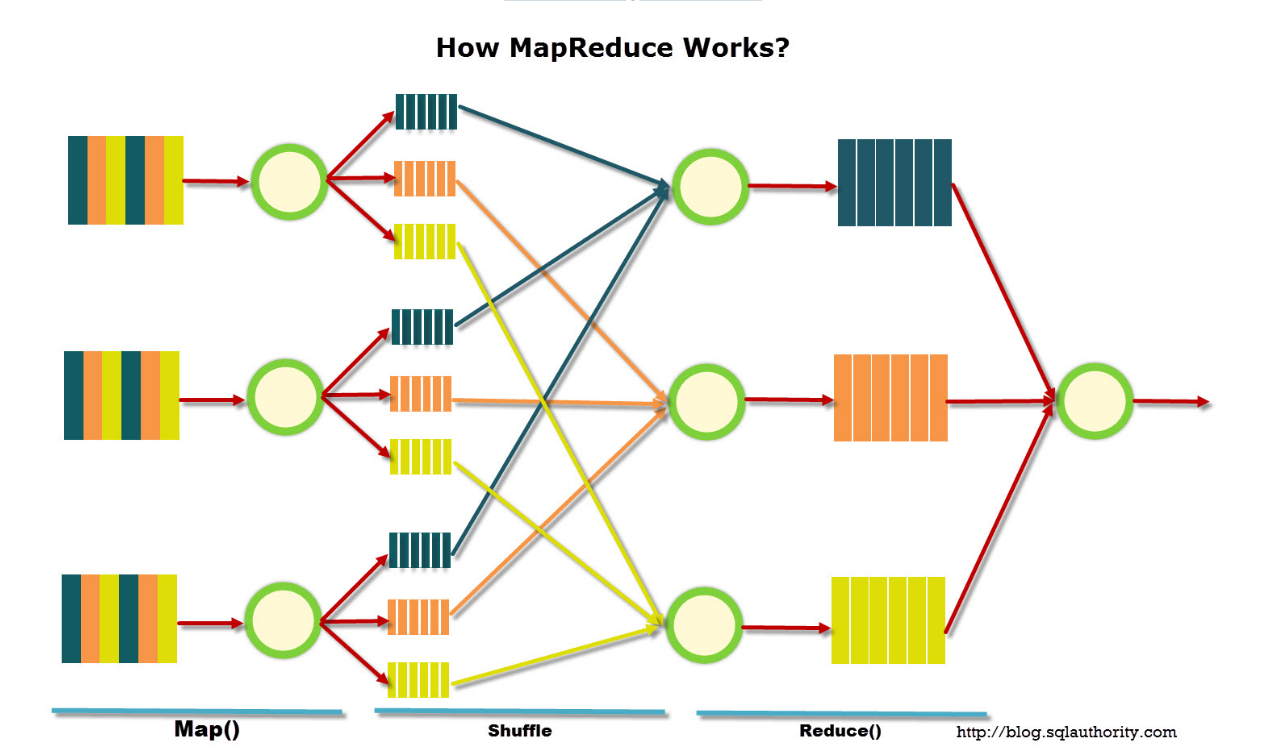
\includegraphics[width=\textwidth]{src/images/big-data/map-reduce.png}
    \centering
\end{figure}

\subsubsection{Platform}
\begin{itemize}
    \item \textit{Schedule}: we need a scheduler that allocates resources for mappers and reducers. Typically we have one master and many workers. The master considers the locality of data when assigning a task to  mapper in order to preserve network bandwidth and task are assigned to workers dynamically.
    \item \textit{Data distribution}: in order to move data from mappers to reducers we need a infrastructure able to do that in a efficient way.
    \item \textit{Fault tolerance}: we need a system that transparently handles the crash of one or more nodes
    \begin{itemize}
        \item \textit{Worker failure:} the master detects failure via periodic heartbeats. When a worker failure is detected, both completed and in-progress map tasks on that worker should be re-executed. On the contrary, only in-progress reduce tasks on that worker should be re-executed. This because completed reduce tasks have already wrote in the distributed file system.
        \item \textit{Master failure:} since the system state is check-pointed and saved in the \textit{GFS (Global File System)}, a new master recovers and continues from the last known state.\\
        Note that, if we have \textit{stragglers}, so tasks that take long time to execute, we need to reschedule any remaining executing task.
    \end{itemize}
\end{itemize}

\subsubsection{Strengths, limitations and typical applications}
\paragraph{Strengths}
\begin{itemize}
    \item The developers write simple functions
    \item The system manages complexity of allocation and synchronization
    \item Good approach when we have to deal with large-scale data analysis
\end{itemize}

\paragraph{Limitation}
\begin{itemize}
    \item Very high overhead
    \item Lower raw performance than \textit{HCP (High Performance Computing}
    \item Very fixed and rigid paradigm (the next step cannot start if the previous one is completed)
\end{itemize}

\paragraph{Typical applications}
\begin{itemize}
    \item Sequence of steps, each requiring map and reduce
    \item Series of data transformations
    \item \textit{"Iterating until reach convergence"} problems
\end{itemize}